
\section{Caching}
Aufgrund der Entscheidung alle Daten Verlustfrei im Originalformat zu speichern sowie der Verwendung von In-Memory Tabellen-artigen Datenstrukturen, muss sichergestellt werden, dass nicht bei jeder Operation die Originaldaten von Format-Parser neu eingelesen werden müssen.

Aus diesem Grund wurde ein dreistufiges Caching-Konzept für die gesamte Applikation implementiert. Es werden die Caching-Mechanismen von Django mit eingen Modifikationen/Erweiterungen verwendet. Aus diesem Grund können die Caching-Backends jederzeit durch beliebige von Django Unterstützte Backends wie z.B. Memcached, Filesystem, etc. verwendet werden.

\subsection{Caches}

\xxx[ref]
\begin{figure}[H]
\centering
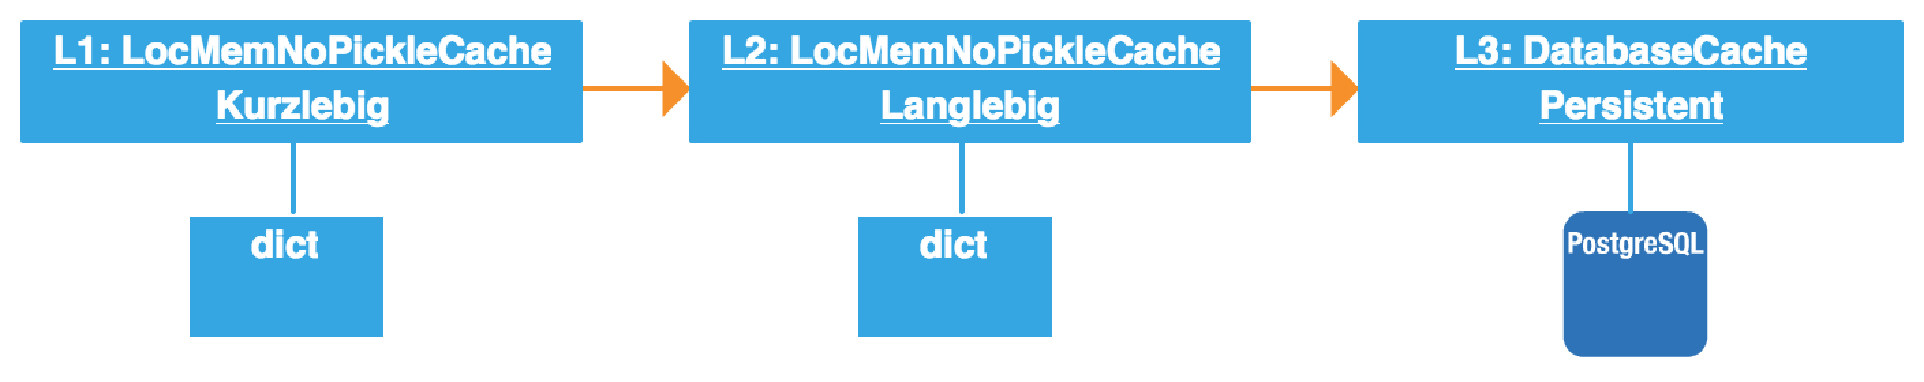
\includegraphics[width=\linewidth]{fig/caching.pdf}
\caption{Übersicht der Caches}
\label{fig:pd:caches}
\end{figure}

\xxx[ref]
\mytable{lX}{
  \textbf{Cache} & \textbf{Beschreibung}\\
  \midrule
  Level 1 & Der Level 1 Cache ist ein In-Memory Cache der Applikation und sehr kurzlebig (\SI{60}{\second}). Dieser wird hauptsächlich verwenden um Zwischenresultate wie Formatkonversionen oder Resultate einer Abfrage zu speichern, damit der Benutzer im Webfrontend die Daten sofort mittels Pagination anschauen kann.\\

  Level 2 & Im Cache zweiter Stufe werden hauptsächlich Daten des Level 3 Caches für mehrere Minuten zwischengespeichert um den Overhead der Abfrage inkl. potenziellem Transfer mehrerer Megabytes sowie Deserialisierung der Python Objekte aus der Datenbank zu vermeiden.\\

  Level 3 & Im persistenten Cache werden eingelesene Dateien im intermediären Format (d.h. DataFrame Objekte) sowie gespeicherte Transformationen ohne Online-Datenquellen persistiert.\\
}{Beschreibung der Caches}{pd:caches}

\subsection{Invalidierung}
\xxx[fscala: cache key]